\documentclass[twoside]{book}

% Packages required by doxygen
\usepackage{fixltx2e}
\usepackage{calc}
\usepackage{doxygen}
\usepackage[export]{adjustbox} % also loads graphicx
\usepackage{graphicx}
\usepackage[utf8]{inputenc}
\usepackage{makeidx}
\usepackage{multicol}
\usepackage{multirow}
\PassOptionsToPackage{warn}{textcomp}
\usepackage{textcomp}
\usepackage[nointegrals]{wasysym}
\usepackage[table]{xcolor}

% Font selection
\usepackage[T1]{fontenc}
\usepackage[scaled=.90]{helvet}
\usepackage{courier}
\usepackage{amssymb}
\usepackage{sectsty}
\renewcommand{\familydefault}{\sfdefault}
\allsectionsfont{%
  \fontseries{bc}\selectfont%
  \color{darkgray}%
}
\renewcommand{\DoxyLabelFont}{%
  \fontseries{bc}\selectfont%
  \color{darkgray}%
}
\newcommand{\+}{\discretionary{\mbox{\scriptsize$\hookleftarrow$}}{}{}}

% Page & text layout
\usepackage{geometry}
\geometry{%
  a4paper,%
  top=2.5cm,%
  bottom=2.5cm,%
  left=2.5cm,%
  right=2.5cm%
}
\tolerance=750
\hfuzz=15pt
\hbadness=750
\setlength{\emergencystretch}{15pt}
\setlength{\parindent}{0cm}
\setlength{\parskip}{0.2cm}
\makeatletter
\renewcommand{\paragraph}{%
  \@startsection{paragraph}{4}{0ex}{-1.0ex}{1.0ex}{%
    \normalfont\normalsize\bfseries\SS@parafont%
  }%
}
\renewcommand{\subparagraph}{%
  \@startsection{subparagraph}{5}{0ex}{-1.0ex}{1.0ex}{%
    \normalfont\normalsize\bfseries\SS@subparafont%
  }%
}
\makeatother

% Headers & footers
\usepackage{fancyhdr}
\pagestyle{fancyplain}
\fancyhead[LE]{\fancyplain{}{\bfseries\thepage}}
\fancyhead[CE]{\fancyplain{}{}}
\fancyhead[RE]{\fancyplain{}{\bfseries\leftmark}}
\fancyhead[LO]{\fancyplain{}{\bfseries\rightmark}}
\fancyhead[CO]{\fancyplain{}{}}
\fancyhead[RO]{\fancyplain{}{\bfseries\thepage}}
\fancyfoot[LE]{\fancyplain{}{}}
\fancyfoot[CE]{\fancyplain{}{}}
\fancyfoot[RE]{\fancyplain{}{\bfseries\scriptsize Generated on Fri Oct 2 2015 13\+:41\+:54 for Chess2720 by Doxygen }}
\fancyfoot[LO]{\fancyplain{}{\bfseries\scriptsize Generated on Fri Oct 2 2015 13\+:41\+:54 for Chess2720 by Doxygen }}
\fancyfoot[CO]{\fancyplain{}{}}
\fancyfoot[RO]{\fancyplain{}{}}
\renewcommand{\footrulewidth}{0.4pt}
\renewcommand{\chaptermark}[1]{%
  \markboth{#1}{}%
}
\renewcommand{\sectionmark}[1]{%
  \markright{\thesection\ #1}%
}

% Indices & bibliography
\usepackage{natbib}
\usepackage[titles]{tocloft}
\setcounter{tocdepth}{3}
\setcounter{secnumdepth}{5}
\makeindex

% Hyperlinks (required, but should be loaded last)
\usepackage{ifpdf}
\ifpdf
  \usepackage[pdftex,pagebackref=true]{hyperref}
\else
  \usepackage[ps2pdf,pagebackref=true]{hyperref}
\fi
\hypersetup{%
  colorlinks=true,%
  linkcolor=blue,%
  citecolor=blue,%
  unicode%
}

% Custom commands
\newcommand{\clearemptydoublepage}{%
  \newpage{\pagestyle{empty}\cleardoublepage}%
}


%===== C O N T E N T S =====

\begin{document}

% Titlepage & ToC
\hypersetup{pageanchor=false,
             bookmarks=true,
             bookmarksnumbered=true,
             pdfencoding=unicode
            }
\pagenumbering{roman}
\begin{titlepage}
\vspace*{7cm}
\begin{center}%
{\Large Chess2720 \\[1ex]\large 0.\+1 }\\
\vspace*{1cm}
{\large Generated by Doxygen 1.8.10}\\
\vspace*{0.5cm}
{\small Fri Oct 2 2015 13:41:54}\\
\end{center}
\end{titlepage}
\clearemptydoublepage
\tableofcontents
\clearemptydoublepage
\pagenumbering{arabic}
\hypersetup{pageanchor=true}

%--- Begin generated contents ---
\chapter{Hierarchical Index}
\section{Class Hierarchy}
This inheritance list is sorted roughly, but not completely, alphabetically\+:\begin{DoxyCompactList}
\item \contentsline{section}{Board}{\pageref{classBoard}}{}
\item \contentsline{section}{Chess2720}{\pageref{classChess2720}}{}
\item \contentsline{section}{Game}{\pageref{classGame}}{}
\begin{DoxyCompactList}
\item \contentsline{section}{Chess}{\pageref{classChess}}{}
\end{DoxyCompactList}
\item \contentsline{section}{Piece}{\pageref{classPiece}}{}
\item \contentsline{section}{Square}{\pageref{classSquare}}{}
\end{DoxyCompactList}

\chapter{Class Index}
\section{Class List}
Here are the classes, structs, unions and interfaces with brief descriptions\+:\begin{DoxyCompactList}
\item\contentsline{section}{\hyperlink{classBoard}{Board} }{\pageref{classBoard}}{}
\item\contentsline{section}{\hyperlink{classChess}{Chess} }{\pageref{classChess}}{}
\item\contentsline{section}{\hyperlink{classChess2720}{Chess2720} }{\pageref{classChess2720}}{}
\item\contentsline{section}{\hyperlink{classGame}{Game} \\*\+: An abstraction of a board game. The game has a \hyperlink{classBoard}{Board} }{\pageref{classGame}}{}
\item\contentsline{section}{\hyperlink{classPiece}{Piece} }{\pageref{classPiece}}{}
\item\contentsline{section}{\hyperlink{classSquare}{Square} \\*\+: \hyperlink{classSquare}{Square} is a location on the board that can contain a \hyperlink{classPiece}{Piece} and its location info ie. row and column }{\pageref{classSquare}}{}
\end{DoxyCompactList}

\chapter{File Index}
\section{File List}
Here is a list of all files with brief descriptions\+:\begin{DoxyCompactList}
\item\contentsline{section}{\hyperlink{Board_8cpp}{Board.\+cpp} }{\pageref{Board_8cpp}}{}
\item\contentsline{section}{\hyperlink{Board_8h}{Board.\+h} }{\pageref{Board_8h}}{}
\item\contentsline{section}{\hyperlink{Chess_8cpp}{Chess.\+cpp} }{\pageref{Chess_8cpp}}{}
\item\contentsline{section}{\hyperlink{Chess_8h}{Chess.\+h} }{\pageref{Chess_8h}}{}
\item\contentsline{section}{\hyperlink{Chess2720_8cpp}{Chess2720.\+cpp} }{\pageref{Chess2720_8cpp}}{}
\item\contentsline{section}{\hyperlink{Chess2720_8h}{Chess2720.\+h} }{\pageref{Chess2720_8h}}{}
\item\contentsline{section}{\hyperlink{Game_8cpp}{Game.\+cpp} }{\pageref{Game_8cpp}}{}
\item\contentsline{section}{\hyperlink{Game_8h}{Game.\+h} }{\pageref{Game_8h}}{}
\item\contentsline{section}{\hyperlink{Piece_8cpp}{Piece.\+cpp} }{\pageref{Piece_8cpp}}{}
\item\contentsline{section}{\hyperlink{Piece_8h}{Piece.\+h} }{\pageref{Piece_8h}}{}
\item\contentsline{section}{\hyperlink{Square_8cpp}{Square.\+cpp} }{\pageref{Square_8cpp}}{}
\item\contentsline{section}{\hyperlink{Square_8h}{Square.\+h} }{\pageref{Square_8h}}{}
\end{DoxyCompactList}

\chapter{Class Documentation}
\hypertarget{classBoard}{}\section{Board Class Reference}
\label{classBoard}\index{Board@{Board}}
\subsection*{Public Member Functions}
\begin{DoxyCompactItemize}
\item 
\hyperlink{classBoard_a1291ca893864123e2a144ce5e4d8beb3}{Board} (int height, int width)
\item 
void \hyperlink{classBoard_a07010bc149d198961c4669cec2ca4905}{draw} (ostream $\ast$o)
\item 
void \hyperlink{classBoard_ab96f988bdac00e84aa3ae9995e16921c}{place\+Piece} (\hyperlink{classPiece}{Piece} $\ast$p, \hyperlink{classSquare}{Square} $\ast$s)
\item 
void \hyperlink{classBoard_a71bbcd990439137e81b14ab229787daa}{move\+Piece} (\hyperlink{classSquare}{Square} $\ast$s, \hyperlink{classSquare}{Square} $\ast$d)
\item 
\hypertarget{classBoard_afa30630891e15327329bd1fb62de3484}{}\hyperlink{classSquare}{Square} $\ast$ {\bfseries get\+Square} (int r, int c)\label{classBoard_afa30630891e15327329bd1fb62de3484}

\end{DoxyCompactItemize}
\subsection*{Public Attributes}
\begin{DoxyCompactItemize}
\item 
\hypertarget{classBoard_aa0cb8de0254520dc08dab5796643c8e5}{}int {\bfseries height}\label{classBoard_aa0cb8de0254520dc08dab5796643c8e5}

\item 
\hypertarget{classBoard_a90a8efaa4736af25511ac948bdd27d6c}{}int {\bfseries width}\label{classBoard_a90a8efaa4736af25511ac948bdd27d6c}

\item 
\hypertarget{classBoard_a7a0a34a623e8fd5e350fdb31bd10f182}{}vector$<$ \hyperlink{classSquare}{Square} $\ast$ $>$ {\bfseries squares}\label{classBoard_a7a0a34a623e8fd5e350fdb31bd10f182}

\end{DoxyCompactItemize}


\subsection{Constructor \& Destructor Documentation}
\hypertarget{classBoard_a1291ca893864123e2a144ce5e4d8beb3}{}\index{Board@{Board}!Board@{Board}}
\index{Board@{Board}!Board@{Board}}
\subsubsection[{Board(int height, int width)}]{\setlength{\rightskip}{0pt plus 5cm}Board\+::\+Board (
\begin{DoxyParamCaption}
\item[{int}]{height, }
\item[{int}]{width}
\end{DoxyParamCaption}
)}\label{classBoard_a1291ca893864123e2a144ce5e4d8beb3}
Constructor\+: takes two parameters – width and height – for specifying the size of the board. 

\subsection{Member Function Documentation}
\hypertarget{classBoard_a07010bc149d198961c4669cec2ca4905}{}\index{Board@{Board}!draw@{draw}}
\index{draw@{draw}!Board@{Board}}
\subsubsection[{draw(ostream $\ast$o)}]{\setlength{\rightskip}{0pt plus 5cm}void Board\+::draw (
\begin{DoxyParamCaption}
\item[{ostream $\ast$}]{o}
\end{DoxyParamCaption}
)}\label{classBoard_a07010bc149d198961c4669cec2ca4905}
Draws the board to an output stream \hypertarget{classBoard_a71bbcd990439137e81b14ab229787daa}{}\index{Board@{Board}!move\+Piece@{move\+Piece}}
\index{move\+Piece@{move\+Piece}!Board@{Board}}
\subsubsection[{move\+Piece(\+Square $\ast$s, Square $\ast$d)}]{\setlength{\rightskip}{0pt plus 5cm}void Board\+::move\+Piece (
\begin{DoxyParamCaption}
\item[{{\bf Square} $\ast$}]{s, }
\item[{{\bf Square} $\ast$}]{d}
\end{DoxyParamCaption}
)}\label{classBoard_a71bbcd990439137e81b14ab229787daa}
Moves the \hyperlink{classPiece}{Piece} on \hyperlink{classSquare}{Square} s to \hyperlink{classSquare}{Square} d \hypertarget{classBoard_ab96f988bdac00e84aa3ae9995e16921c}{}\index{Board@{Board}!place\+Piece@{place\+Piece}}
\index{place\+Piece@{place\+Piece}!Board@{Board}}
\subsubsection[{place\+Piece(\+Piece $\ast$p, Square $\ast$s)}]{\setlength{\rightskip}{0pt plus 5cm}void Board\+::place\+Piece (
\begin{DoxyParamCaption}
\item[{{\bf Piece} $\ast$}]{p, }
\item[{{\bf Square} $\ast$}]{s}
\end{DoxyParamCaption}
)}\label{classBoard_ab96f988bdac00e84aa3ae9995e16921c}
Places a \hyperlink{classPiece}{Piece} on a \hyperlink{classSquare}{Square} 

The documentation for this class was generated from the following files\+:\begin{DoxyCompactItemize}
\item 
Board.\+h\item 
Board.\+cpp\end{DoxyCompactItemize}

\hypertarget{classChess}{}\section{Chess Class Reference}
\label{classChess}\index{Chess@{Chess}}
Inheritance diagram for Chess\+:\begin{figure}[H]
\begin{center}
\leavevmode
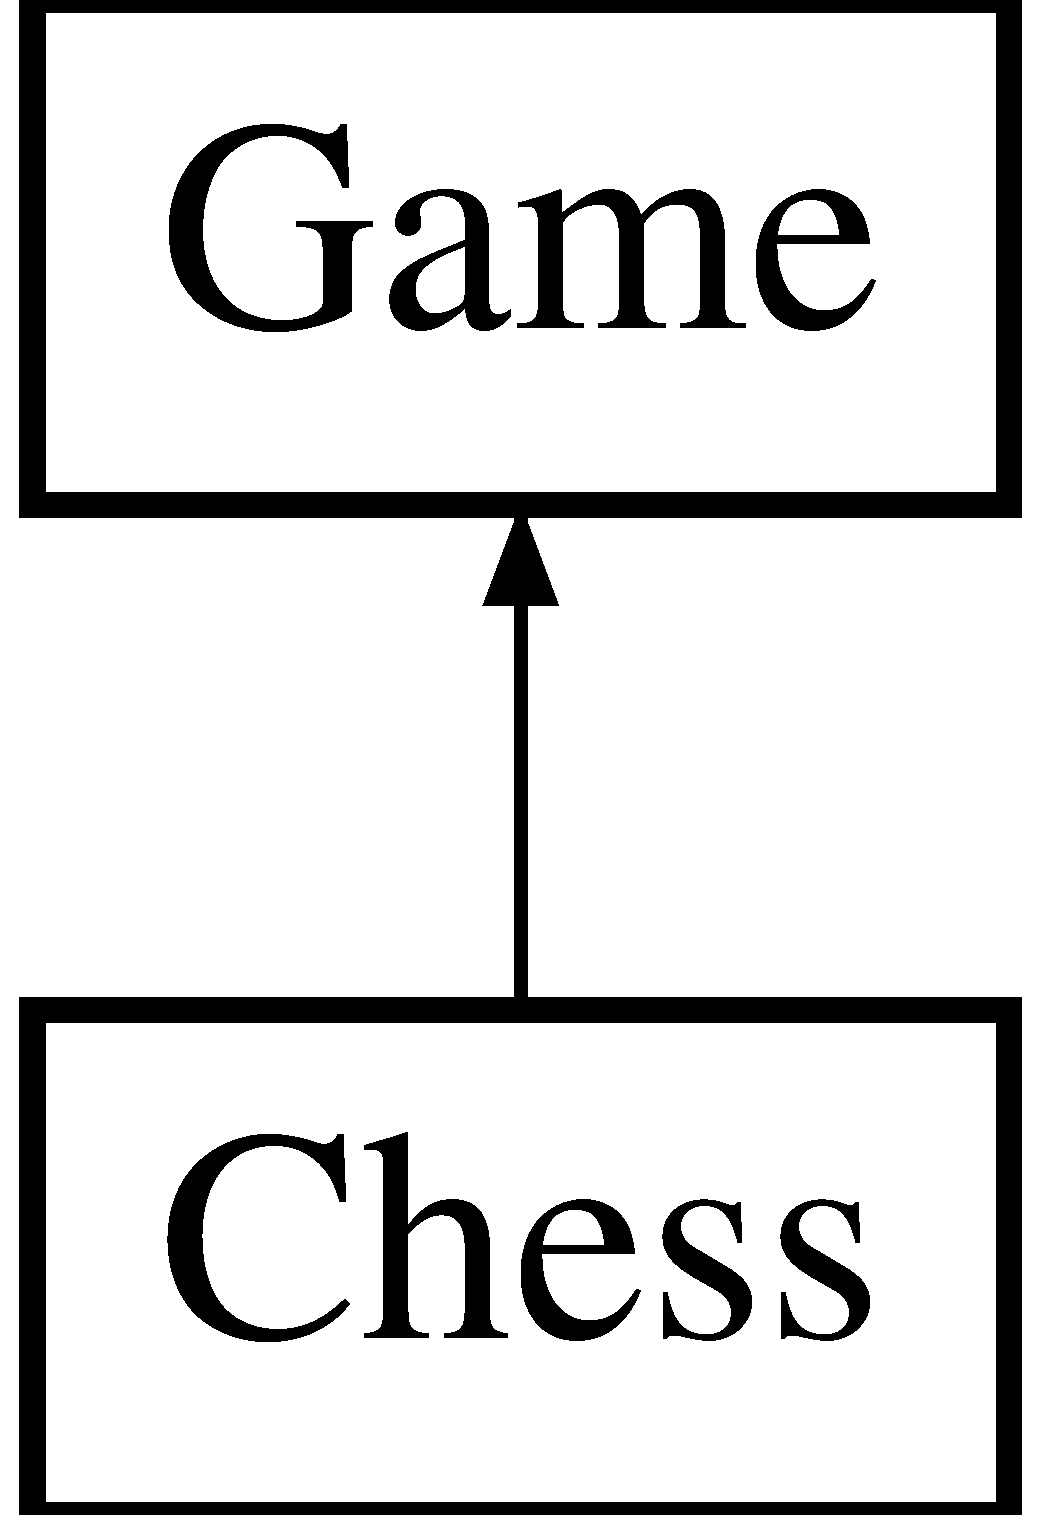
\includegraphics[height=2.000000cm]{classChess}
\end{center}
\end{figure}
\subsection*{Public Member Functions}
\begin{DoxyCompactItemize}
\item 
\hyperlink{classChess_a8b493f742d0ceced6f853fa30d3c05a8}{Chess} ()
\item 
void \hyperlink{classChess_a9722d5c13c442eae33ca17792996213a}{setup} ()
\item 
bool \hyperlink{classChess_ac85e41b8580d3300185bd2bc264ec6d8}{is\+Over} ()
\item 
\hyperlink{classSquare}{Square} $\ast$ \hyperlink{classChess_a8266d0da94f72df7991799790915e38b}{get\+Square} (istream \&is)
\end{DoxyCompactItemize}
\subsection*{Additional Inherited Members}


\subsection{Constructor \& Destructor Documentation}
\hypertarget{classChess_a8b493f742d0ceced6f853fa30d3c05a8}{}\index{Chess@{Chess}!Chess@{Chess}}
\index{Chess@{Chess}!Chess@{Chess}}
\subsubsection[{Chess()}]{\setlength{\rightskip}{0pt plus 5cm}Chess\+::\+Chess (
\begin{DoxyParamCaption}
{}
\end{DoxyParamCaption}
)}\label{classChess_a8b493f742d0ceced6f853fa30d3c05a8}
Constructor\+: Creates a 6x6 chess board and the pieces. alternative maybe char char\+Pieces \mbox{[}\mbox{]} = \{\textquotesingle{}r\textquotesingle{},\textquotesingle{}b\textquotesingle{},\textquotesingle{}k\textquotesingle{},\textquotesingle{}q\textquotesingle{},\textquotesingle{}b\textquotesingle{},\textquotesingle{}r\textquotesingle{},\textquotesingle{}p\textquotesingle{},\textquotesingle{}p\textquotesingle{},\textquotesingle{}p\textquotesingle{},\textquotesingle{}p\textquotesingle{},\textquotesingle{}p\textquotesingle{},\textquotesingle{}p\textquotesingle{}\}; pieces(char\+Pieces, char\+Pieces + sizeof(char\+Pieces) / sizeof(char));

\subsection{Member Function Documentation}
\hypertarget{classChess_a8266d0da94f72df7991799790915e38b}{}\index{Chess@{Chess}!get\+Square@{get\+Square}}
\index{get\+Square@{get\+Square}!Chess@{Chess}}
\subsubsection[{get\+Square(istream \&is)}]{\setlength{\rightskip}{0pt plus 5cm}{\bf Square} $\ast$ Chess\+::get\+Square (
\begin{DoxyParamCaption}
\item[{istream \&}]{is}
\end{DoxyParamCaption}
)\hspace{0.3cm}{\ttfamily [virtual]}}\label{classChess_a8266d0da94f72df7991799790915e38b}
Reads the row and column for a location on the board. The row and column values are separated by a space on one line. 

Implements \hyperlink{classGame_a36fc5e6874822115ff6685c608da50db}{Game}.

\hypertarget{classChess_ac85e41b8580d3300185bd2bc264ec6d8}{}\index{Chess@{Chess}!is\+Over@{is\+Over}}
\index{is\+Over@{is\+Over}!Chess@{Chess}}
\subsubsection[{is\+Over()}]{\setlength{\rightskip}{0pt plus 5cm}bool Chess\+::is\+Over (
\begin{DoxyParamCaption}
{}
\end{DoxyParamCaption}
)\hspace{0.3cm}{\ttfamily [virtual]}}\label{classChess_ac85e41b8580d3300185bd2bc264ec6d8}
Overrides the \hyperlink{classChess_ac85e41b8580d3300185bd2bc264ec6d8}{is\+Over()} function from \hyperlink{classGame}{Game} to indicate that the game ends when one of the King pieces is taken. 

Implements \hyperlink{classGame_ae3f5006e677b713fa7f85d906cde3dde}{Game}.

\hypertarget{classChess_a9722d5c13c442eae33ca17792996213a}{}\index{Chess@{Chess}!setup@{setup}}
\index{setup@{setup}!Chess@{Chess}}
\subsubsection[{setup()}]{\setlength{\rightskip}{0pt plus 5cm}void Chess\+::setup (
\begin{DoxyParamCaption}
{}
\end{DoxyParamCaption}
)\hspace{0.3cm}{\ttfamily [virtual]}}\label{classChess_a9722d5c13c442eae33ca17792996213a}
Overrides the \hyperlink{classChess_a9722d5c13c442eae33ca17792996213a}{setup()} function from \hyperlink{classGame}{Game} to populate the board with the pieces. 

Implements \hyperlink{classGame_a49067dcf360cfe353b9a99910136ac26}{Game}.



The documentation for this class was generated from the following files\+:\begin{DoxyCompactItemize}
\item 
Chess.\+h\item 
Chess.\+cpp\end{DoxyCompactItemize}

\hypertarget{classChess2720}{}\section{Chess2720 Class Reference}
\label{classChess2720}\index{Chess2720@{Chess2720}}


{\ttfamily \#include $<$Chess2720.\+h$>$}

\subsection*{Public Member Functions}
\begin{DoxyCompactItemize}
\item 
\hypertarget{classChess2720_a8c8732303f01d9fa4bef9922f74e0636}{}int {\bfseries main} ()\label{classChess2720_a8c8732303f01d9fa4bef9922f74e0636}

\end{DoxyCompactItemize}


\subsection{Detailed Description}
\hyperlink{Chess2720_8h_source}{Chess2720.\+h}

Created on\+: Oct 1, 2015 Author\+: root 

The documentation for this class was generated from the following file\+:\begin{DoxyCompactItemize}
\item 
Chess2720.\+h\end{DoxyCompactItemize}

\hypertarget{classGame}{}\section{Game Class Reference}
\label{classGame}\index{Game@{Game}}


\+: An abstraction of a board game. The game has a \hyperlink{classBoard}{Board}.  




{\ttfamily \#include $<$Game.\+h$>$}

Inheritance diagram for Game\+:\begin{figure}[H]
\begin{center}
\leavevmode
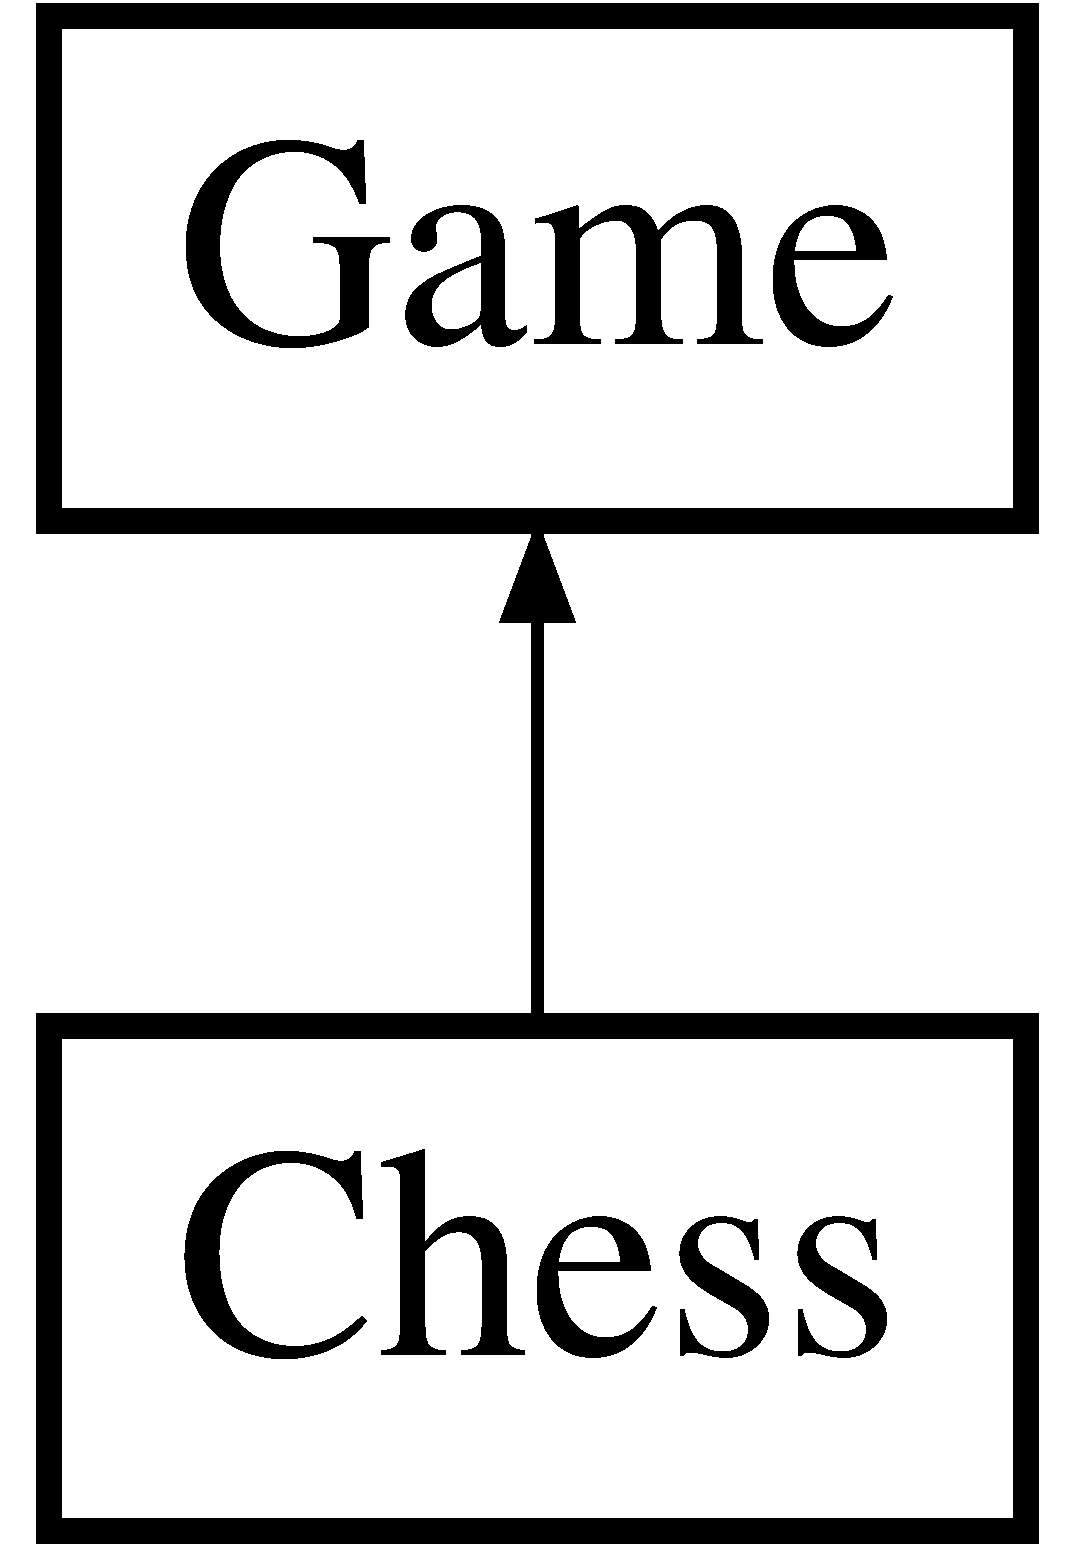
\includegraphics[height=2.000000cm]{classGame}
\end{center}
\end{figure}
\subsection*{Public Member Functions}
\begin{DoxyCompactItemize}
\item 
void \hyperlink{classGame_aa333825d0bca80e91e53c7e23f053405}{play} ()
\item 
virtual void \hyperlink{classGame_a49067dcf360cfe353b9a99910136ac26}{setup} ()=0
\item 
virtual bool \hyperlink{classGame_aa07345e2f71668d147c0ed2257ed0e50}{is\+Over} () const  =0
\item 
virtual \hyperlink{classSquare}{Square} $\ast$ \hyperlink{classGame_a78d07b6a2cedd5150b856cfa41a087da}{get\+Square} (istream const \&is)=0
\item 
virtual \hyperlink{classGame_ae3d112ca6e0e55150d2fdbc704474530}{$\sim$\+Game} ()
\end{DoxyCompactItemize}
\subsection*{Public Attributes}
\begin{DoxyCompactItemize}
\item 
bool \hyperlink{classGame_ae82939826eff0a8847cb822cf95227f4}{over}
\item 
\hyperlink{classBoard}{Board} $\ast$ \hyperlink{classGame_ae38e501e177586af48d2e2300b6be4ba}{board}
\end{DoxyCompactItemize}


\subsection{Detailed Description}
\+: An abstraction of a board game. The game has a \hyperlink{classBoard}{Board}. 

\begin{DoxyAuthor}{Author}
\+: Amrit 
\end{DoxyAuthor}


\subsection{Constructor \& Destructor Documentation}
\hypertarget{classGame_ae3d112ca6e0e55150d2fdbc704474530}{}\index{Game@{Game}!````~Game@{$\sim$\+Game}}
\index{````~Game@{$\sim$\+Game}!Game@{Game}}
\subsubsection[{$\sim$\+Game()}]{\setlength{\rightskip}{0pt plus 5cm}Game\+::$\sim$\+Game (
\begin{DoxyParamCaption}
{}
\end{DoxyParamCaption}
)\hspace{0.3cm}{\ttfamily [virtual]}}\label{classGame_ae3d112ca6e0e55150d2fdbc704474530}


\subsection{Member Function Documentation}
\hypertarget{classGame_a78d07b6a2cedd5150b856cfa41a087da}{}\index{Game@{Game}!get\+Square@{get\+Square}}
\index{get\+Square@{get\+Square}!Game@{Game}}
\subsubsection[{get\+Square(istream const \&is)=0}]{\setlength{\rightskip}{0pt plus 5cm}virtual {\bf Square}$\ast$ Game\+::get\+Square (
\begin{DoxyParamCaption}
\item[{istream const \&}]{is}
\end{DoxyParamCaption}
)\hspace{0.3cm}{\ttfamily [pure virtual]}}\label{classGame_a78d07b6a2cedd5150b856cfa41a087da}
reads the input stream and returns a square from the board. 

Implemented in \hyperlink{classChess_a48b59dcf880ff97114b8c5a3989b0364}{Chess}.

\hypertarget{classGame_aa07345e2f71668d147c0ed2257ed0e50}{}\index{Game@{Game}!is\+Over@{is\+Over}}
\index{is\+Over@{is\+Over}!Game@{Game}}
\subsubsection[{is\+Over() const  =0}]{\setlength{\rightskip}{0pt plus 5cm}virtual bool Game\+::is\+Over (
\begin{DoxyParamCaption}
{}
\end{DoxyParamCaption}
) const\hspace{0.3cm}{\ttfamily [pure virtual]}}\label{classGame_aa07345e2f71668d147c0ed2257ed0e50}
Indicates if the game is over. \begin{DoxyReturn}{Returns}
bool 
\end{DoxyReturn}


Implemented in \hyperlink{classChess_a62b09f4b86c385c8042b8c7e192e10e5}{Chess}.

\hypertarget{classGame_aa333825d0bca80e91e53c7e23f053405}{}\index{Game@{Game}!play@{play}}
\index{play@{play}!Game@{Game}}
\subsubsection[{play()}]{\setlength{\rightskip}{0pt plus 5cm}void Game\+::play (
\begin{DoxyParamCaption}
{}
\end{DoxyParamCaption}
)}\label{classGame_aa333825d0bca80e91e53c7e23f053405}
\hypertarget{classGame_a49067dcf360cfe353b9a99910136ac26}{}\index{Game@{Game}!setup@{setup}}
\index{setup@{setup}!Game@{Game}}
\subsubsection[{setup()=0}]{\setlength{\rightskip}{0pt plus 5cm}virtual void Game\+::setup (
\begin{DoxyParamCaption}
{}
\end{DoxyParamCaption}
)\hspace{0.3cm}{\ttfamily [pure virtual]}}\label{classGame_a49067dcf360cfe353b9a99910136ac26}
Setups up the board for the game. 

Implemented in \hyperlink{classChess_a9722d5c13c442eae33ca17792996213a}{Chess}.



\subsection{Member Data Documentation}
\hypertarget{classGame_ae38e501e177586af48d2e2300b6be4ba}{}\index{Game@{Game}!board@{board}}
\index{board@{board}!Game@{Game}}
\subsubsection[{board}]{\setlength{\rightskip}{0pt plus 5cm}{\bf Board}$\ast$ Game\+::board}\label{classGame_ae38e501e177586af48d2e2300b6be4ba}
\hypertarget{classGame_ae82939826eff0a8847cb822cf95227f4}{}\index{Game@{Game}!over@{over}}
\index{over@{over}!Game@{Game}}
\subsubsection[{over}]{\setlength{\rightskip}{0pt plus 5cm}bool Game\+::over}\label{classGame_ae82939826eff0a8847cb822cf95227f4}


The documentation for this class was generated from the following files\+:\begin{DoxyCompactItemize}
\item 
\hyperlink{Game_8h}{Game.\+h}\item 
\hyperlink{Game_8cpp}{Game.\+cpp}\end{DoxyCompactItemize}

\hypertarget{classPiece}{}\section{Piece Class Reference}
\label{classPiece}\index{Piece@{Piece}}


{\ttfamily \#include $<$Piece.\+h$>$}

\subsection*{Public Member Functions}
\begin{DoxyCompactItemize}
\item 
\hyperlink{classPiece_ad9009085b915df6c20503f2ce144c931}{Piece} (string \hyperlink{classPiece_aa789cfb1749a0dc7ae40c20e369a4321}{colour}, char \hyperlink{classPiece_a00143ae55b69981ae484cc7521b6d81a}{symbol})
\begin{DoxyCompactList}\small\item\em \+: This cpp file provides constructor for \hyperlink{classPiece}{Piece} and implements \hyperlink{classPiece_a9f6a89d6fd5ae865af73c2220d1a5839}{is\+Alive()} and \hyperlink{classPiece_a4c2ace5bc3eb68e46e8599702b782d94}{kill()} \end{DoxyCompactList}\item 
bool \hyperlink{classPiece_a9f6a89d6fd5ae865af73c2220d1a5839}{is\+Alive} ()
\item 
void \hyperlink{classPiece_a4c2ace5bc3eb68e46e8599702b782d94}{kill} ()
\item 
\hyperlink{classPiece_a5d7a4f6bade94cb33b6f634de8aa7918}{$\sim$\+Piece} ()
\end{DoxyCompactItemize}
\subsection*{Public Attributes}
\begin{DoxyCompactItemize}
\item 
string \hyperlink{classPiece_aa789cfb1749a0dc7ae40c20e369a4321}{colour}
\item 
char \hyperlink{classPiece_a00143ae55b69981ae484cc7521b6d81a}{symbol}
\item 
bool \hyperlink{classPiece_a8b3c2f812ead74ba513f521e63f767f9}{alive}
\end{DoxyCompactItemize}


\subsection{Constructor \& Destructor Documentation}
\hypertarget{classPiece_ad9009085b915df6c20503f2ce144c931}{}\index{Piece@{Piece}!Piece@{Piece}}
\index{Piece@{Piece}!Piece@{Piece}}
\subsubsection[{Piece(string colour, char symbol)}]{\setlength{\rightskip}{0pt plus 5cm}Piece\+::\+Piece (
\begin{DoxyParamCaption}
\item[{string}]{colour, }
\item[{char}]{symbol}
\end{DoxyParamCaption}
)}\label{classPiece_ad9009085b915df6c20503f2ce144c931}


\+: This cpp file provides constructor for \hyperlink{classPiece}{Piece} and implements \hyperlink{classPiece_a9f6a89d6fd5ae865af73c2220d1a5839}{is\+Alive()} and \hyperlink{classPiece_a4c2ace5bc3eb68e46e8599702b782d94}{kill()} 

Didn\textquotesingle{}t include the variable alive in the constructor since everything at the beginning of the game will be alive when pieces are created.

\+: Amrit Grewal \hypertarget{classPiece_a5d7a4f6bade94cb33b6f634de8aa7918}{}\index{Piece@{Piece}!````~Piece@{$\sim$\+Piece}}
\index{````~Piece@{$\sim$\+Piece}!Piece@{Piece}}
\subsubsection[{$\sim$\+Piece()}]{\setlength{\rightskip}{0pt plus 5cm}Piece\+::$\sim$\+Piece (
\begin{DoxyParamCaption}
{}
\end{DoxyParamCaption}
)}\label{classPiece_a5d7a4f6bade94cb33b6f634de8aa7918}


\subsection{Member Function Documentation}
\hypertarget{classPiece_a9f6a89d6fd5ae865af73c2220d1a5839}{}\index{Piece@{Piece}!is\+Alive@{is\+Alive}}
\index{is\+Alive@{is\+Alive}!Piece@{Piece}}
\subsubsection[{is\+Alive()}]{\setlength{\rightskip}{0pt plus 5cm}bool Piece\+::is\+Alive (
\begin{DoxyParamCaption}
{}
\end{DoxyParamCaption}
)}\label{classPiece_a9f6a89d6fd5ae865af73c2220d1a5839}
Returns true if the piece is still active on the board, false otherwise \hypertarget{classPiece_a4c2ace5bc3eb68e46e8599702b782d94}{}\index{Piece@{Piece}!kill@{kill}}
\index{kill@{kill}!Piece@{Piece}}
\subsubsection[{kill()}]{\setlength{\rightskip}{0pt plus 5cm}void Piece\+::kill (
\begin{DoxyParamCaption}
{}
\end{DoxyParamCaption}
)}\label{classPiece_a4c2ace5bc3eb68e46e8599702b782d94}
sets the piece to be inactive on the board 

\subsection{Member Data Documentation}
\hypertarget{classPiece_a8b3c2f812ead74ba513f521e63f767f9}{}\index{Piece@{Piece}!alive@{alive}}
\index{alive@{alive}!Piece@{Piece}}
\subsubsection[{alive}]{\setlength{\rightskip}{0pt plus 5cm}bool Piece\+::alive}\label{classPiece_a8b3c2f812ead74ba513f521e63f767f9}
\hypertarget{classPiece_aa789cfb1749a0dc7ae40c20e369a4321}{}\index{Piece@{Piece}!colour@{colour}}
\index{colour@{colour}!Piece@{Piece}}
\subsubsection[{colour}]{\setlength{\rightskip}{0pt plus 5cm}string Piece\+::colour}\label{classPiece_aa789cfb1749a0dc7ae40c20e369a4321}
\hypertarget{classPiece_a00143ae55b69981ae484cc7521b6d81a}{}\index{Piece@{Piece}!symbol@{symbol}}
\index{symbol@{symbol}!Piece@{Piece}}
\subsubsection[{symbol}]{\setlength{\rightskip}{0pt plus 5cm}char Piece\+::symbol}\label{classPiece_a00143ae55b69981ae484cc7521b6d81a}


The documentation for this class was generated from the following files\+:\begin{DoxyCompactItemize}
\item 
\hyperlink{Piece_8h}{Piece.\+h}\item 
\hyperlink{Piece_8cpp}{Piece.\+cpp}\end{DoxyCompactItemize}

\hypertarget{classSquare}{}\section{Square Class Reference}
\label{classSquare}\index{Square@{Square}}


\+: \hyperlink{classSquare}{Square} is a location on the board that can contain a \hyperlink{classPiece}{Piece} and its location info ie. row and column.  




{\ttfamily \#include $<$Square.\+h$>$}

\subsection*{Public Member Functions}
\begin{DoxyCompactItemize}
\item 
\hyperlink{classSquare_a2fafe3d65a3b4166f1fe8b6540db2199}{Square} (int \hyperlink{classSquare_aa353950a9ef437401db55ae605b0f8b9}{row}, int \hyperlink{classSquare_a08d4af37ead0391bec8f9cbaff083da0}{col})
\item 
char \hyperlink{classSquare_aadadc7c924a6f07fd13d271118e65a16}{symbol} () const 
\item 
void \hyperlink{classSquare_a7cf9aa874fea67f6a9056cad15752ab2}{set\+Piece} (\hyperlink{classPiece}{Piece} $\ast$p)
\item 
\hyperlink{classPiece}{Piece} $\ast$ \hyperlink{classSquare_ab5b0c359853874b38c17bbe0b3f6aadf}{get\+Piece} () const 
\item 
\hyperlink{classPiece}{Piece} $\ast$ \hyperlink{classSquare_a21ec1e5b9fb287c33f911ef032443503}{remove\+Piece} ()
\item 
\hyperlink{classSquare_a90af7ce1060cff7b717ceddb333846b8}{$\sim$\+Square} ()
\end{DoxyCompactItemize}
\subsection*{Public Attributes}
\begin{DoxyCompactItemize}
\item 
\hyperlink{classPiece}{Piece} $\ast$ \hyperlink{classSquare_a52eab334fb3f4fe8d29f1f1b7570a52f}{piece}
\item 
int \hyperlink{classSquare_aa353950a9ef437401db55ae605b0f8b9}{row}
\item 
int \hyperlink{classSquare_a08d4af37ead0391bec8f9cbaff083da0}{col}
\end{DoxyCompactItemize}


\subsection{Detailed Description}
\+: \hyperlink{classSquare}{Square} is a location on the board that can contain a \hyperlink{classPiece}{Piece} and its location info ie. row and column. 

\begin{DoxyAuthor}{Author}
\+: Amrit 
\end{DoxyAuthor}


\subsection{Constructor \& Destructor Documentation}
\hypertarget{classSquare_a2fafe3d65a3b4166f1fe8b6540db2199}{}\index{Square@{Square}!Square@{Square}}
\index{Square@{Square}!Square@{Square}}
\subsubsection[{Square(int row, int col)}]{\setlength{\rightskip}{0pt plus 5cm}Square\+::\+Square (
\begin{DoxyParamCaption}
\item[{int}]{row, }
\item[{int}]{col}
\end{DoxyParamCaption}
)}\label{classSquare_a2fafe3d65a3b4166f1fe8b6540db2199}
Constructor\+: takes two parameters – row and column – for specifying the location of the square on the board. \hypertarget{classSquare_a90af7ce1060cff7b717ceddb333846b8}{}\index{Square@{Square}!````~Square@{$\sim$\+Square}}
\index{````~Square@{$\sim$\+Square}!Square@{Square}}
\subsubsection[{$\sim$\+Square()}]{\setlength{\rightskip}{0pt plus 5cm}Square\+::$\sim$\+Square (
\begin{DoxyParamCaption}
{}
\end{DoxyParamCaption}
)}\label{classSquare_a90af7ce1060cff7b717ceddb333846b8}
Destructor 

\subsection{Member Function Documentation}
\hypertarget{classSquare_ab5b0c359853874b38c17bbe0b3f6aadf}{}\index{Square@{Square}!get\+Piece@{get\+Piece}}
\index{get\+Piece@{get\+Piece}!Square@{Square}}
\subsubsection[{get\+Piece() const }]{\setlength{\rightskip}{0pt plus 5cm}{\bf Piece} $\ast$ Square\+::get\+Piece (
\begin{DoxyParamCaption}
{}
\end{DoxyParamCaption}
) const}\label{classSquare_ab5b0c359853874b38c17bbe0b3f6aadf}
Returns the piece on the square, if it exists, otherwise returns N\+U\+L\+L; \hypertarget{classSquare_a21ec1e5b9fb287c33f911ef032443503}{}\index{Square@{Square}!remove\+Piece@{remove\+Piece}}
\index{remove\+Piece@{remove\+Piece}!Square@{Square}}
\subsubsection[{remove\+Piece()}]{\setlength{\rightskip}{0pt plus 5cm}{\bf Piece} $\ast$ Square\+::remove\+Piece (
\begin{DoxyParamCaption}
{}
\end{DoxyParamCaption}
)}\label{classSquare_a21ec1e5b9fb287c33f911ef032443503}
Removes a piece from a square and returns it, if it exists. \hypertarget{classSquare_a7cf9aa874fea67f6a9056cad15752ab2}{}\index{Square@{Square}!set\+Piece@{set\+Piece}}
\index{set\+Piece@{set\+Piece}!Square@{Square}}
\subsubsection[{set\+Piece(\+Piece $\ast$p)}]{\setlength{\rightskip}{0pt plus 5cm}void Square\+::set\+Piece (
\begin{DoxyParamCaption}
\item[{{\bf Piece} $\ast$}]{p}
\end{DoxyParamCaption}
)}\label{classSquare_a7cf9aa874fea67f6a9056cad15752ab2}
Sets a piece on the square \hypertarget{classSquare_aadadc7c924a6f07fd13d271118e65a16}{}\index{Square@{Square}!symbol@{symbol}}
\index{symbol@{symbol}!Square@{Square}}
\subsubsection[{symbol() const }]{\setlength{\rightskip}{0pt plus 5cm}char Square\+::symbol (
\begin{DoxyParamCaption}
{}
\end{DoxyParamCaption}
) const}\label{classSquare_aadadc7c924a6f07fd13d271118e65a16}
Returns the symbol of the piece on the square, or a symbol indicating an empty square (“.\+”). 

\subsection{Member Data Documentation}
\hypertarget{classSquare_a08d4af37ead0391bec8f9cbaff083da0}{}\index{Square@{Square}!col@{col}}
\index{col@{col}!Square@{Square}}
\subsubsection[{col}]{\setlength{\rightskip}{0pt plus 5cm}int Square\+::col}\label{classSquare_a08d4af37ead0391bec8f9cbaff083da0}
\hypertarget{classSquare_a52eab334fb3f4fe8d29f1f1b7570a52f}{}\index{Square@{Square}!piece@{piece}}
\index{piece@{piece}!Square@{Square}}
\subsubsection[{piece}]{\setlength{\rightskip}{0pt plus 5cm}{\bf Piece}$\ast$ Square\+::piece}\label{classSquare_a52eab334fb3f4fe8d29f1f1b7570a52f}
\hypertarget{classSquare_aa353950a9ef437401db55ae605b0f8b9}{}\index{Square@{Square}!row@{row}}
\index{row@{row}!Square@{Square}}
\subsubsection[{row}]{\setlength{\rightskip}{0pt plus 5cm}int Square\+::row}\label{classSquare_aa353950a9ef437401db55ae605b0f8b9}


The documentation for this class was generated from the following files\+:\begin{DoxyCompactItemize}
\item 
\hyperlink{Square_8h}{Square.\+h}\item 
\hyperlink{Square_8cpp}{Square.\+cpp}\end{DoxyCompactItemize}

\chapter{File Documentation}
\hypertarget{Board_8cpp}{}\section{Board.\+cpp File Reference}
\label{Board_8cpp}\index{Board.\+cpp@{Board.\+cpp}}
{\ttfamily \#include \char`\"{}Board.\+h\char`\"{}}\\*

\hypertarget{Board_8h}{}\section{Board.\+h File Reference}
\label{Board_8h}\index{Board.\+h@{Board.\+h}}
{\ttfamily \#include \char`\"{}Chess.\+h\char`\"{}}\\*
{\ttfamily \#include \char`\"{}Piece.\+h\char`\"{}}\\*
{\ttfamily \#include \char`\"{}Square.\+h\char`\"{}}\\*
{\ttfamily \#include $<$iostream$>$}\\*
{\ttfamily \#include $<$vector$>$}\\*
\subsection*{Classes}
\begin{DoxyCompactItemize}
\item 
class \hyperlink{classBoard}{Board}
\end{DoxyCompactItemize}

\hypertarget{Chess_8cpp}{}\section{Chess.\+cpp File Reference}
\label{Chess_8cpp}\index{Chess.\+cpp@{Chess.\+cpp}}
{\ttfamily \#include \char`\"{}Chess.\+h\char`\"{}}\\*
\subsection*{Functions}
\begin{DoxyCompactItemize}
\item 
Chess\+:: \hyperlink{Chess_8cpp_ad4b2ab6672e32319ee3781d6d431837f}{$\sim$\+Chess} ()
\end{DoxyCompactItemize}


\subsection{Function Documentation}
\hypertarget{Chess_8cpp_ad4b2ab6672e32319ee3781d6d431837f}{}\index{Chess.\+cpp@{Chess.\+cpp}!````~Chess@{$\sim$\+Chess}}
\index{````~Chess@{$\sim$\+Chess}!Chess.\+cpp@{Chess.\+cpp}}
\subsubsection[{$\sim$\+Chess()}]{\setlength{\rightskip}{0pt plus 5cm}Chess\+:: $\sim${\bf Chess} (
\begin{DoxyParamCaption}
{}
\end{DoxyParamCaption}
)}\label{Chess_8cpp_ad4b2ab6672e32319ee3781d6d431837f}

\hypertarget{Chess_8h}{}\section{Chess.\+h File Reference}
\label{Chess_8h}\index{Chess.\+h@{Chess.\+h}}
{\ttfamily \#include \char`\"{}Board.\+h\char`\"{}}\\*
{\ttfamily \#include \char`\"{}Game.\+h\char`\"{}}\\*
{\ttfamily \#include \char`\"{}Square.\+h\char`\"{}}\\*
{\ttfamily \#include $<$iostream$>$}\\*
{\ttfamily \#include $<$vector$>$}\\*
\subsection*{Classes}
\begin{DoxyCompactItemize}
\item 
class \hyperlink{classChess}{Chess}
\end{DoxyCompactItemize}

\hypertarget{Chess2720_8cpp}{}\section{Chess2720.\+cpp File Reference}
\label{Chess2720_8cpp}\index{Chess2720.\+cpp@{Chess2720.\+cpp}}
{\ttfamily \#include \char`\"{}Chess.\+h\char`\"{}}\\*
{\ttfamily \#include \char`\"{}Chess2720.\+h\char`\"{}}\\*
\subsection*{Functions}
\begin{DoxyCompactItemize}
\item 
int \hyperlink{Chess2720_8cpp_ae66f6b31b5ad750f1fe042a706a4e3d4}{main} ()
\end{DoxyCompactItemize}


\subsection{Function Documentation}
\hypertarget{Chess2720_8cpp_ae66f6b31b5ad750f1fe042a706a4e3d4}{}\index{Chess2720.\+cpp@{Chess2720.\+cpp}!main@{main}}
\index{main@{main}!Chess2720.\+cpp@{Chess2720.\+cpp}}
\subsubsection[{main()}]{\setlength{\rightskip}{0pt plus 5cm}int main (
\begin{DoxyParamCaption}
{}
\end{DoxyParamCaption}
)}\label{Chess2720_8cpp_ae66f6b31b5ad750f1fe042a706a4e3d4}
\hyperlink{Chess2720_8cpp}{Chess2720.\+cpp}

Created on\+: Oct 1, 2015 Author\+: root 
\hypertarget{Chess2720_8h}{}\section{Chess2720.\+h File Reference}
\label{Chess2720_8h}\index{Chess2720.\+h@{Chess2720.\+h}}
\subsection*{Classes}
\begin{DoxyCompactItemize}
\item 
class \hyperlink{classChess2720}{Chess2720}
\end{DoxyCompactItemize}

\hypertarget{Game_8cpp}{}\section{Game.\+cpp File Reference}
\label{Game_8cpp}\index{Game.\+cpp@{Game.\+cpp}}
{\ttfamily \#include \char`\"{}Game.\+h\char`\"{}}\\*

\hypertarget{Game_8h}{}\section{Game.\+h File Reference}
\label{Game_8h}\index{Game.\+h@{Game.\+h}}
{\ttfamily \#include \char`\"{}Square.\+h\char`\"{}}\\*
{\ttfamily \#include $<$iostream$>$}\\*
\subsection*{Classes}
\begin{DoxyCompactItemize}
\item 
class \hyperlink{classGame}{Game}
\begin{DoxyCompactList}\small\item\em \+: An abstraction of a board game. The game has a \hyperlink{classBoard}{Board}. \end{DoxyCompactList}\end{DoxyCompactItemize}

\hypertarget{Piece_8cpp}{}\section{Piece.\+cpp File Reference}
\label{Piece_8cpp}\index{Piece.\+cpp@{Piece.\+cpp}}
{\ttfamily \#include \char`\"{}Piece.\+h\char`\"{}}\\*

\hypertarget{Piece_8h}{}\section{Piece.\+h File Reference}
\label{Piece_8h}\index{Piece.\+h@{Piece.\+h}}
{\ttfamily \#include $<$string$>$}\\*
\subsection*{Classes}
\begin{DoxyCompactItemize}
\item 
class \hyperlink{classPiece}{Piece}
\end{DoxyCompactItemize}

\hypertarget{Square_8cpp}{}\section{Square.\+cpp File Reference}
\label{Square_8cpp}\index{Square.\+cpp@{Square.\+cpp}}
{\ttfamily \#include \char`\"{}Square.\+h\char`\"{}}\\*

\hypertarget{Square_8h}{}\section{Square.\+h File Reference}
\label{Square_8h}\index{Square.\+h@{Square.\+h}}
{\ttfamily \#include \char`\"{}Piece.\+h\char`\"{}}\\*
\subsection*{Classes}
\begin{DoxyCompactItemize}
\item 
class \hyperlink{classSquare}{Square}
\begin{DoxyCompactList}\small\item\em \+: \hyperlink{classSquare}{Square} is a location on the board that can contain a \hyperlink{classPiece}{Piece} and its location info ie. row and column. \end{DoxyCompactList}\end{DoxyCompactItemize}

%--- End generated contents ---

% Index
\backmatter
\newpage
\phantomsection
\clearemptydoublepage
\addcontentsline{toc}{chapter}{Index}
\printindex

\end{document}
